\begin{frame}
\frametitle{Thrombolysis in subgroups of patients (predicted use in a common 10k cohort at each team)}

\footnotesize The range of the predicted thrombolysis use across the 132 hospitals for subsets of the 10k patient cohort. The subsets of patients to the right of \emph{Ideal patients} all have the ideal patient characteristics with the specified changes

\begin{center}
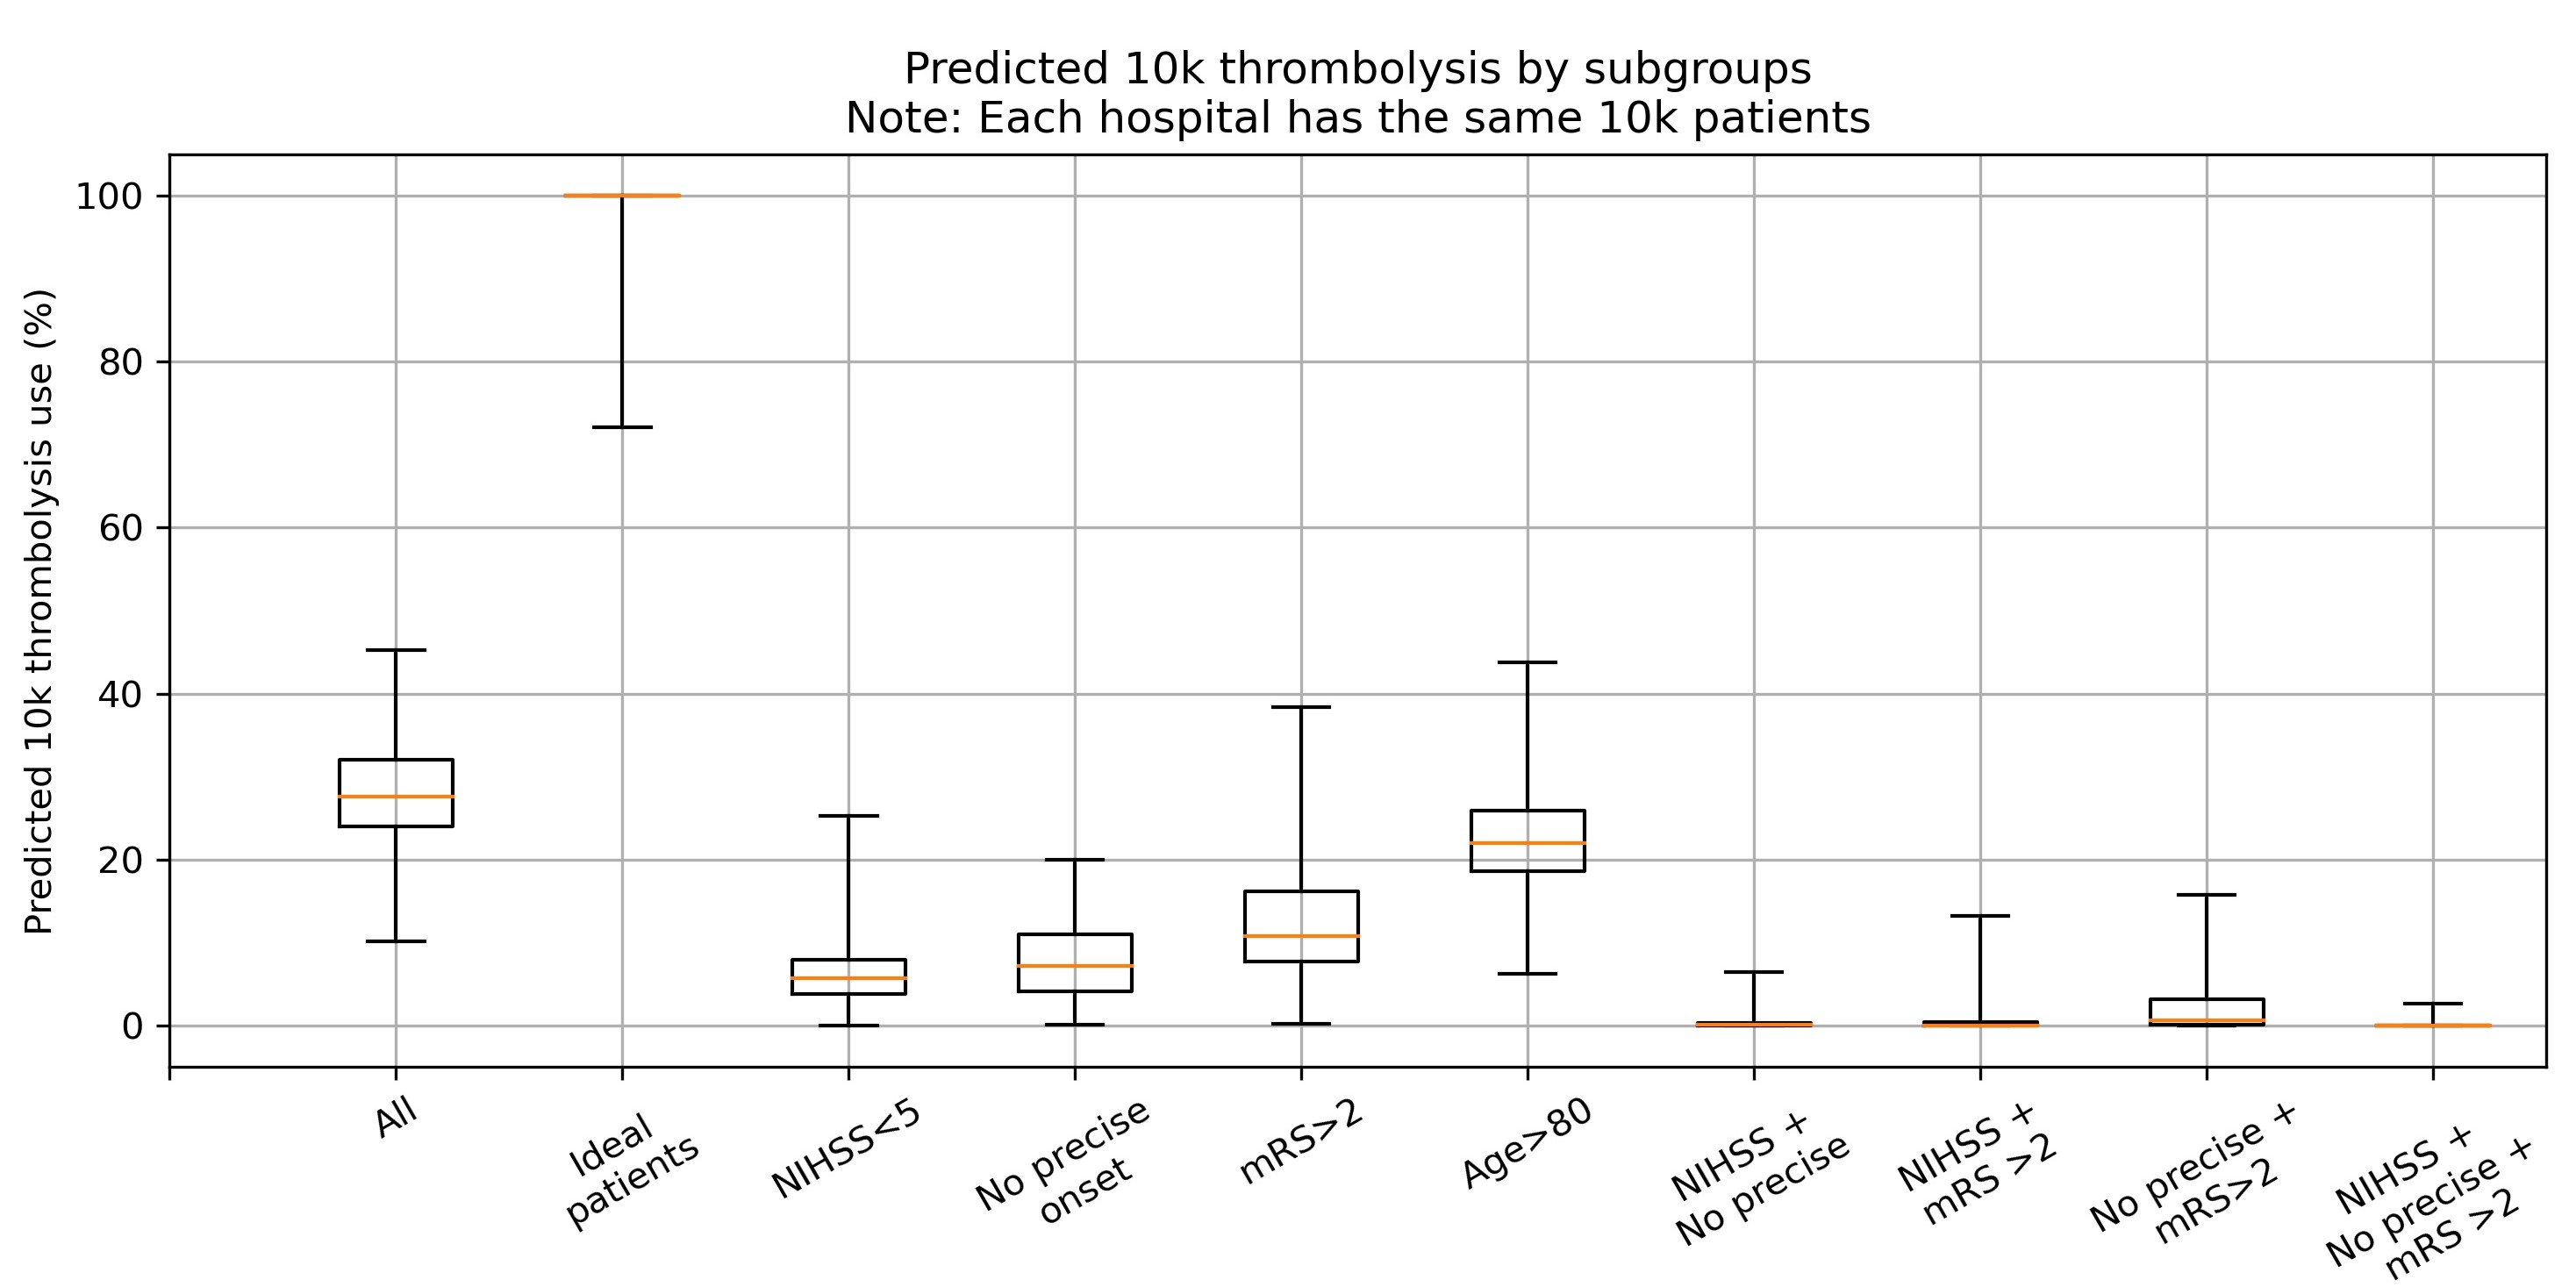
\includegraphics[width=0.83\textwidth]{./images/15c_modelled_subgroup_violin.jpg}
\end{center}

\scriptsize An \emph{ideal patient} has: Stroke severity NIHSS in range 10-25, Arrival-to-scan time \textless{} 20 minutes, Stroke type = infarction, Precise onset time = True, Prior disability level (mRS) = 0, No use of AF anticoagulants, Onset-to-arrival time \textless{} 90 minutes, Age \textless{80 years}, Onset during sleep = False
\end{frame}